%% GeneDiseaseTrace-LLM: manuscript for the Journal of Biomedical Informatics.
%% Layout and section logic follow a recent JBI paper prepared with elsarticle
%% (Park et al., "Automated Identification of Incidentalomas Requiring Follow-Up", arXiv:2512.05537).
%% Build: latexmk -pdf main.tex
\documentclass[preprint,10pt,letterpaper]{elsarticle}

\usepackage[T1]{fontenc}
\usepackage[utf8]{inputenc}
\usepackage{lmodern}
\usepackage[letterpaper,hmargin=1.35in,vmargin=1.1in]{geometry}   % text block of the model paper
\usepackage{microtype}
\usepackage{amsmath,amssymb}
\usepackage{booktabs,tabularx,multirow,array}
\usepackage{xcolor}
\usepackage{graphicx}
\usepackage[hidelinks]{hyperref}
\usepackage{enumitem}
\setlist{nosep}
\setlength{\emergencystretch}{3em}
\renewcommand{\topfraction}{0.9}
\renewcommand{\floatpagefraction}{0.8}
% Shared palette and TikZ/pgfplots settings for all figures (loaded by main.tex
% and graphical_abstract.tex). Colours are colour-blind safe (Okabe-Ito based).
\usepackage{tikz}
\usepackage{pgfplots}
\pgfplotsset{compat=1.18}
\usepgfplotslibrary{groupplots}
\usetikzlibrary{arrows.meta,positioning,fit,backgrounds,calc,shapes.misc,decorations.pathreplacing}

% Systems
\definecolor{ours}{HTML}{0B5CAD}      % our method (Claude Opus 5.5)
\definecolor{gpt}{HTML}{009E73}       % our method with GPT-6.1 Sol
\definecolor{pubtator}{HTML}{D55E00}  % PubTator3
% Entities
\definecolor{genefill}{HTML}{DCEBFA}
\definecolor{geneline}{HTML}{0B5CAD}
\definecolor{disfill}{HTML}{FBE3D6}
\definecolor{disline}{HTML}{C2410C}
% Statuses
\definecolor{stsup}{HTML}{1B7F4B}
\definecolor{stunc}{HTML}{C98A00}
\definecolor{stneg}{HTML}{B4233C}
\definecolor{stnf}{HTML}{8A8F98}
% Neutrals
\definecolor{ink}{HTML}{1F2933}
\definecolor{muted}{HTML}{6B7280}
\definecolor{rule}{HTML}{D1D5DB}
\definecolor{panel}{HTML}{F5F7FA}

\tikzset{
  panel/.style={draw=rule, fill=panel, rounded corners=3pt, inner sep=6pt},
  paneltitle/.style={font=\sffamily\bfseries\small, text=ink, anchor=north west},
  gene/.style={fill=genefill, draw=geneline, rounded corners=1.5pt, inner sep=1.6pt, font=\sffamily\scriptsize},
  dis/.style={fill=disfill, draw=disline, rounded corners=1.5pt, inner sep=1.6pt, font=\sffamily\scriptsize},
  badge/.style={rounded corners=2pt, inner sep=1.8pt, font=\sffamily\tiny\bfseries, text=white},
  flow/.style={-{Stealth[length=2.2mm]}, line width=0.9pt, draw=ink},
}
% Inline highlights inside text nodes
\newcommand{\hlgene}[1]{\tikz[baseline=(g.base)]\node[fill=genefill, inner sep=0.6pt, rounded corners=1pt] (g) {\strut #1};}
\newcommand{\hldis}[1]{\tikz[baseline=(d.base)]\node[fill=disfill, inner sep=0.6pt, rounded corners=1pt] (d) {\strut #1};}
\newcommand{\sid}[1]{{\ttfamily\color{muted}\tiny[#1]}}
\newcommand{\badge}[2]{\tikz[baseline=(b.base)]\node[badge, fill=#1] (b) {#2};}

\pgfplotsset{
  gdt/.style={
    font=\sffamily\scriptsize,
    tick label style={font=\sffamily\tiny},
    label style={font=\sffamily\scriptsize},
    title style={font=\sffamily\bfseries\scriptsize, align=center},
    axis line style={draw=muted},
    tick style={draw=muted},
    major grid style={draw=rule!70, line width=0.3pt},
    grid=major,
  },
}


\newcommand{\st}[1]{\texttt{#1}}             % status and reason-code names
\newcommand{\todo}[1]{\textcolor{stneg}{[TODO: #1]}}

\journal{Journal of Biomedical Informatics}

\begin{document}

\begin{frontmatter}

\title{Evidence-Traceable, Status-Aware Gene--Disease Relation Extraction with a Large Language Model: A Multi-Benchmark Evaluation}

\author[a]{Zeqian Tong}
\author[b]{\todo{co-authors}}
\affiliation[a]{organization={\todo{affiliation}}}
\affiliation[b]{organization={\todo{affiliation}}}

\begin{abstract}
\setlength{\parindent}{0pt}\setlength{\parskip}{6pt}%
\textbf{Objective:} Current relation extractors return positive entity pairs, mostly from abstracts, without supporting text, certainty levels, or study-versus-background provenance. We developed and evaluated a zero-shot method that extracts gene--disease relations from abstracts and full texts together with sentence-level evidence, a four-way status (\st{supported}, \st{uncertain}, \st{explicit\_negative}, \st{not\_found}), and a source label (this study or background).

\textbf{Methods:} In a single request per paper, a large language model (Claude Opus 5.5) follows a frozen one-page decision card and cites supporting sentences by ID; a deterministic validator checks every cited span against source text. Without benchmark-specific tuning, we evaluated the method on BioRED (419 abstracts), EU-ADR (100 abstracts), and 40 RENET2 full-text articles using pair matching, bootstrap confidence intervals, and PubTator3 as comparator.

\textbf{Results:} On BioRED, strict precision was 0.894 (95\% CI 0.855--0.931) and recall 0.430. On a 50-abstract test sample, in-domain PubTator3 scored higher (F1 0.726 vs 0.551), while both systems recovered 73\% of gold relations. On EU-ADR, F1 was comparable (0.506 vs 0.529) and all three negative gold pairs were labelled \st{explicit\_negative}. On RENET2 full texts, our recall exceeded PubTator3's (0.370 vs 0.254), and only 2 of 223 \st{supported} pairs contradicted a gold label. Re-querying 97 unjudged same-sentence BioRED pairs yielded no new \st{supported} relation, showing that misses were not overlooked; instead, routing \st{uncertain} pairs by reason code (chosen on Train+Dev) raised held-out Test F1 from 0.542 to 0.627 without precision loss (0.846 vs 0.853). GPT-6.1 Sol gave the same F1 (0.555), at USD 0.056 per abstract and USD 0.44 per full text.

\textbf{Conclusion:} A written decision card with deterministic validation turns a general-purpose LLM into a precise, auditable gene--disease extractor that complements supervised tools. Its recall gap mainly reflects a stricter evidence standard than benchmark annotators apply, and status labels let users adjust this trade-off.
\end{abstract}

\begin{keyword}
Relation Extraction; Gene--Disease Association; Large Language Models; Biocuration; Evidence Traceability
\end{keyword}

\end{frontmatter}

%% ===================================================================
\section{Introduction}

Gene--disease associations underpin variant interpretation, drug-target discovery, and curated knowledge bases such as DisGeNET~\cite{pinero2020disgenet} and CTD~\cite{davis2023ctd}. Because most of this knowledge is published as free text across more than a million new articles a year, manual curation alone cannot keep pace. Automatic relation extraction has therefore advanced steadily on benchmarks such as BioRED~\cite{luo2022biored}: supervised encoders~\cite{lee2020biobert,gu2021pubmedbert,lai2023biorex} and literature-scale systems such as PubTator3~\cite{wei2024pubtator3} now reach high F1 in their training domain.

Yet a substantial gap remains between benchmark relation extraction and practical biocuration. Current tools return a flat list of positive pairs, mostly from abstracts, whereas curation requires richer, auditable records across the full text. First, curators must see supporting sentences to check each claim in seconds. Second, a paper may support a relation, hedge it, or report no association; collapsing these into ``related'' or ``not related'' discards negative and speculative findings. Third, curators distinguish a paper's own results from citations of prior work. Finally, abstract-only tools miss relations stated only in the body: in our 100-paper full-text corpus, 90\% of supported relations had evidence only outside the abstract.

Large language models (LLMs) can read full papers and follow written instructions, making them natural candidates for this richer task. Applying LLMs to curation, however, faces both a reliability challenge and an evaluation challenge. Brief, free-form prompts leave boundary cases undefined and can produce unverified text spans or invalid schemas~\cite{chen2025benchmarking,wadhwa2023revisiting}, whereas multi-turn agent pipelines require multiple costly requests per paper. Meanwhile, benchmark evaluation is difficult when annotation standards differ or gold sets are incomplete, because apparent false positives may be valid relations left unlabelled~\cite{wadhwa2023revisiting,fan2024evaluating}.

We address both challenges in a single-request pipeline: a frozen one-page decision card defines explicit boundary rules, four-way statuses, and source labels; a compact line-based output cites sentence IDs only; and a deterministic validator rejects any answer whose entity mentions or sentence IDs do not match the paper. We evaluate the frozen method across three benchmarks with distinct annotation protocols (BioRED~\cite{luo2022biored}, EU-ADR~\cite{vanmulligen2012euadr}, and RENET2~\cite{su2021renet2}), compare it with PubTator3~\cite{wei2024pubtator3} and GPT-6.1 Sol, and audit contradictions of explicit negative labels separately from unlabelled extra predictions. The method is consistently precise, rarely contradicts explicit negative labels, and owes its recall gap to a stricter evidence standard rather than overlooked text, a trade-off that users can adjust via the status reason codes.

%% ===================================================================
\section{Related Work}

\subsection{Supervised Biomedical Relation Extraction}
Domain-pretrained encoders such as BioBERT~\cite{lee2020biobert} and PubMedBERT~\cite{gu2021pubmedbert}, fine-tuned on annotated corpora, remain the standard approach for biomedical relation extraction. BioREx~\cite{lai2023biorex} improved BioRED performance by pooling heterogeneous corpora during training, and subsequent work added relation directionality~\cite{lai2025directionality}. PubTator3~\cite{wei2024pubtator3} pairs a BioRED-trained relation extractor with entity recognition and normalization across PubMed and PMC, serving as the most widely used public resource and our main comparator. Although effective in their training domain, these supervised systems output only positive relation labels without supporting sentences, certainty levels, or study-versus-background provenance, and PubTator3 extracts relations from abstracts only. Our method addresses each of these curation needs across full texts while complementing supervised extractors.

\subsection{Large Language Models for Relation Extraction and Biocuration}
Recent benchmarks show that zero- and few-shot LLMs lag behind fine-tuned encoders on standard relation extraction metrics~\cite{chen2025benchmarking,islamaj2024biocreative,brokman2025benchmark,gade2025benchmarking}. In the BioCreative VIII BioRED track~\cite{islamaj2024biocreative} and subsequent zero-shot evaluations on BioRED~\cite{brokman2025benchmark} and across 61 biomedical triplet datasets~\cite{gade2025benchmarking}, direct LLM prompting struggled with schema adherence, unaligned entity spans, and ambiguous relation boundaries. Curation frameworks such as SPIRES (OntoGPT)~\cite{caufield2024spires} and DRAGON-AI~\cite{toro2024dragonai} enforce structured templates, but like prior zero-shot studies they use short task prompts and score only positive predictions without verifying cited sentences or grading uncertain and negative findings. Our approach addresses these limitations in three ways: a frozen 1,000-word decision card defines explicit boundary rules and reason codes instead of a brief prompt; line-based output citing sentence IDs is checked verbatim against source text by a deterministic validator; and four-way statuses with source labels capture uncertain, negative, and background assertions alongside supported findings.

\subsection{Gene--Disease Benchmarks and Incomplete Gold Standards}
Gene--disease benchmarks differ substantially in text scope and annotation protocol. BioRED~\cite{luo2022biored} annotates eight relation types between concept pairs in 600 abstracts and marks whether each relation is a new finding (\emph{Novel}). EU-ADR~\cite{vanmulligen2012euadr} labels gene--disease pairs in abstracts as positive, speculative, or negative by annotator consensus. RENET2~\cite{su2021renet2} provides document-level labels on full texts, but only for tool-proposed candidate pairs, with negative labels assigned automatically. Evaluating generative extractors against such corpora is difficult because valid relations are often unannotated: Wadhwa et al.~\cite{wadhwa2023revisiting} showed through manual review that many apparent LLM false positives are valid relations missed by annotators, and Fan et al.~\cite{fan2024evaluating} separated unannotated valid extractions from factual errors. Crowdsourced re-annotation of EU-ADR likewise showed that single-annotator relations and guideline ambiguities account for many disagreements~\cite{li2015crowdsourcing}. To address these protocol differences and incomplete gold sets, we evaluate the same frozen pipeline across all three benchmarks without tuning, use reason codes and source labels to explain disagreements, and audit explicit negative contradictions separately from unlabelled extra predictions.

%% ===================================================================
\section{Methods}

\subsection{Datasets}
We evaluated the method on three public benchmarks that span abstracts and full texts under different annotation protocols (Table~\ref{tab:benchmarks}), supplemented by an unlabelled 100-paper PMC corpus to assess full-text extraction behaviour.

\subsubsection{BioRED}
We used all 419 BioRED abstracts that contain at least one gene--disease relation (Train 275, Dev 71, Test 73), comprising 1,633 gold relations. A relation counts when one endpoint is a gene or gene product and the other is a disease or phenotypic feature, regardless of relation subtype. For the head-to-head comparison with PubTator3, we used a 50-abstract Test sample. Rules for routing \st{uncertain} pairs were selected on Train+Dev only, keeping Test strictly held out.

\subsubsection{EU-ADR}
We used all 100 abstracts of the EU-ADR target--disorder subset, which contains 134 consensus pairs with graded labels: 122 positive (PA), 9 speculative (SA), and 3 negative (NA). Unless stated otherwise, PA pairs serve as gold positive relations, while SA and NA pairs test our status labels.

\subsubsection{RENET2}
We randomly sampled 40 full-text articles from RENET2 (seed 20261028), whose released texts cover the title, abstract, and early body. The sample contains 181 associated, 83 non-associated, and 1 ambiguous pair; non-associated labels were assigned automatically by tools rather than verified by hand. Three associated pairs involve an entity absent from the released text, which we keep in the recall denominator.

\subsubsection{Full-text corpus}
To evaluate full-text extraction beyond abstract-level benchmarks, we ran the pipeline on 100 heterogeneous PMC articles (including research articles, case reports, reviews, and one conference-abstract collection) and compared its output against PubTator3.

\begin{table}[!htbp]
\centering\footnotesize
\caption{Benchmarks used in this study.}
\label{tab:benchmarks}
\begin{tabularx}{\linewidth}{@{}l>{\raggedright\arraybackslash}p{2.3cm}>{\raggedright\arraybackslash}X>{\raggedright\arraybackslash}p{3.4cm}>{\raggedright\arraybackslash}p{2.6cm}@{}}
\toprule
Benchmark & Text & Documents used & Gold gene--disease relations & Labels beyond ``related''\\
\midrule
BioRED~\cite{luo2022biored} & PubMed abstracts & 419 abstracts with $\geq$1 gene--disease relation (Train 275 / Dev 71 / Test 73); 50-abstract Test sample & 1,633 & Novel / not novel\\
EU-ADR~\cite{vanmulligen2012euadr} & PubMed abstracts & Target--disorder subset, 100 abstracts & 134 consensus pairs: 122 PA, 9 SA, 3 NA & Positive / speculative / negative\\
RENET2~\cite{su2021renet2} & PMC full text (title, abstract, early body) & Random sample of 40 articles & 181 associated; 83 non-associated; 1 ambiguous & Non-associated labels tool-assigned\\
\bottomrule
\end{tabularx}
\end{table}

\subsection{Relation Extraction}

\subsubsection{Task Definition}
Given one paper as plain text, the extractor identifies primary gene and disease entities, links each entity to all surface forms that appear verbatim in the text, and assigns one of four statuses to every gene $\times$ disease pair (Table~\ref{tab:status}). Each \st{supported} pair also receives a relation type (causal, correlation, or association) and a source label indicating whether the relation comes from this study, background citations, both, or is unclear. To keep disease endpoints specific, general symptoms and phenotypes are recorded as auxiliary entities rather than primary disease endpoints; Section~\ref{sec:eval} evaluates the impact of this boundary on benchmark recall.

\begin{table}[!htbp]
\centering\footnotesize
\caption{The four pair statuses.}
\label{tab:status}
\begin{tabularx}{\linewidth}{@{}lX@{}}
\toprule
Status & Definition\\
\midrule
\textcolor{stsup}{\st{supported}} & The text reports a finding or an explicit attribution linking the pair (not an aim or a hypothesis), and the link is readable in the text.\\
\textcolor{stunc}{\st{uncertain}} & There is potential evidence, but hedging, scope, identity, co-reference, presupposition or a conflict prevents a decision. A reason code is required.\\
\textcolor{stneg}{\st{explicit\_negative}} & The text explicitly reports no association, or an opposite result, for this pair on a stated question.\\
\textcolor{stnf}{\st{not\_found}} & Everything else, including co-occurrence only. It does not mean the pair is medically unrelated.\\
\bottomrule
\end{tabularx}
\end{table}

\subsubsection{Decision Card}
Our decision rules originated as a detailed annotation guideline refined on development papers prior to any benchmark evaluation. We distilled this guideline into a one-page decision card of about 1,000 words, paired with an output format specification of about 600 words. The card specifies entity typing and merging, the four pair statuses, relation types, source labels, and explicit rules for ambiguous cases: co-occurrence alone is never a relation; authors' speculative statements are labelled \st{uncertain} with reason code \st{hedged\_claim}; variants reported without disease attribution are excluded; and statistical tests support a pair only when they directly test that gene against that disease outcome. The card was frozen as variant V1 before running any benchmark and was never modified across datasets.

Before freezing the card, we compared three prompt variants on a stratified development set of 12 full-text papers that were never used to draft the rules. Condensing the full guideline into the one-page card (V1 vs V2) preserved extraction quality, achieving 0.976 pair-status agreement while reducing first-request cost by about 12\%. Lowering reasoning effort from medium to low (V3) reduced cost by 24\% but missed about 10\% of genes, diseases, and supported relations; we therefore retained medium reasoning effort. \todo{add a minimal-prompt baseline without the card.}

\subsubsection{Single-Request Pipeline}
The extraction pipeline executes four sequential steps per paper (Fig.~\ref{fig:pipeline}). First, in \emph{Packing}, deterministic code splits the paper into numbered blocks and sentences with stable IDs (e.g.\ \texttt{b0012.s3}), removes the reference list, and places the frozen decision card and format specification into a cached system prompt. Second, in \emph{Generation}, a single request to Claude Opus 5.5 (with medium reasoning effort and all tools disabled) produces pipe-separated lines covering entities, evidence items, pair judgments, study findings, conflicts, and rule gaps. Rather than copying quotes, the model cites evidence by sentence ID only, which prevents altered quotations and reduces output tokens. Third, in \emph{Expansion}, a deterministic script matches every predicted surface form verbatim in the text, resolves sentence IDs to exact quotes and character offsets, and constructs the complete gene $\times$ disease matrix by setting unlisted pairs to \st{not\_found}. Fourth, in \emph{Validation}, a deterministic validator checks that every surface form occurs verbatim, every cited sentence ID exists, pair endpoints are primary entities, and all \st{uncertain} pairs carry legal reason codes. Any validation failure triggers a single repair request listing the exact errors. Across the 100-paper full-text corpus, 69 papers passed validation on the first request and 31 required one repair; all 100 passed after repair, and every repair corrected formatting rather than substantive judgments. Fig.~\ref{fig:example} illustrates the complete output for one full-text article.

\begin{figure}[!htbp]
\centering
\resizebox{\linewidth}{!}{% Figure 2. The single-request pipeline. Blue = the one LLM call; grey = deterministic code.
% Counts: experiments/single_shot/README.md (100-paper run); word counts of the frozen V1 card/format.
% Stage boxes hold top-aligned minipages of equal height so their headings line up.
\newcommand{\stagebox}[2]{\begin{minipage}[t][3.05cm][t]{#1}\raggedright #2\end{minipage}}
\begin{tikzpicture}[
  font=\sffamily\scriptsize, text=ink,
  stage/.style={draw=rule, fill=panel, rounded corners=3pt, align=left, inner sep=5pt, anchor=north west},
  llm/.style={stage, draw=ours, fill=genefill, line width=0.8pt},
  io/.style={draw=rule, fill=white, rounded corners=2pt, text width=2.2cm, align=left, inner sep=4pt},
]
% Steps (top-aligned, equal height)
\node[stage] (pack) at (3.3,0) {\stagebox{2.6cm}{%
  {\sffamily\bfseries 1\enspace Packing}\par\smallskip
  Split into blocks and sentences with stable IDs; drop references.\par\smallskip
  {\ttfamily\tiny\color{muted} b0098.s12}\par\smallskip
  Card + format $\rightarrow$ cached system prompt.}};
\node[llm] (gen) at ($(pack.north east)+(0.6,0)$) {\stagebox{3.0cm}{%
  {\sffamily\bfseries\color{ours} 2\enspace One LLM request}\par\smallskip
  Claude Opus 5.5, medium effort, no tools. Returns compact lines that cite sentence IDs only:\par\smallskip
  {\ttfamily\tiny\color{muted} E|G5|gene|MAP3K3|...\\EV|V7|b0098.s12|bg|...\\P|G5|D3|sup|a|bg|...}}};
\node[stage] (exp) at ($(gen.north east)+(0.6,0)$) {\stagebox{2.6cm}{%
  {\sffamily\bfseries 3\enspace Expansion}\par\smallskip
  Locate every surface form verbatim; resolve sentence IDs to quotes and offsets.\par\smallskip
  Build the full gene $\times$ disease matrix; unlisted pairs $\rightarrow$ {\ttfamily not\_found}.}};
\node[stage] (val) at ($(exp.north east)+(0.6,0)$) {\stagebox{2.6cm}{%
  {\sffamily\bfseries 4\enspace Validation}\par\smallskip
  Surface forms occur in the text; sentence IDs exist; endpoints are primary entities; reason codes are legal.}};
% Inputs and output, centred on the step row
\path (pack.west) ++(-0.7,0) coordinate (inmid);
\node[io, anchor=south east] (paper) at ($(inmid)+(0,0.12)$) {\textbf{Paper}\\full text (PMC XML) or abstract};
\node[io, anchor=north east] (card) at ($(inmid)+(0,-0.12)$) {\textbf{Frozen decision card}\\1,044 words, plus output format (594 words)};
\node[io, anchor=west, text width=2.1cm] (out) at ($(val.east)+(0.7,0)$) {\textbf{Traceable output}\\entities and mentions\\evidence quotes\\4-status pair matrix\\bipartite graph};
% Arrows
\draw[flow] (paper.east) -- ++(0.3,0) |- ([yshift=3pt]pack.west);
\draw[flow] (card.east) -- ++(0.3,0) |- ([yshift=-3pt]pack.west);
\draw[flow] (pack) -- (gen);
\draw[flow] (gen) -- (exp);
\draw[flow] (exp) -- (val);
\draw[flow, draw=stsup] (val) -- node[above, font=\sffamily\tiny, text=stsup] {pass} (out);
% Repair loop below the row
\draw[flow, draw=stneg, densely dashed] (val.south) -- ++(0,-0.45) -| (gen.south);
\node[font=\sffamily\tiny, text=stneg, anchor=north] at ($(gen.south)!0.5!(val.south)+(0,-0.5)$)
  {fail $\rightarrow$ one repair request with the error list (31 of 100 papers; all format errors)};
% Legend and totals
\node[anchor=north west, font=\sffamily\tiny, text=muted] at ($(card.south west)+(0,-0.9)$)
  {\textcolor{ours}{\rule{6pt}{6pt}}\,LLM call\quad \textcolor{rule!80!black}{\rule{6pt}{6pt}}\,deterministic code};
\node[anchor=north east, font=\sffamily\tiny, text=muted, align=right] at ($(out.east |- card.south)+(0,-0.9)$)
  {100-paper corpus: 69 pass on the first request, 100 after one repair;\\mean 78\,s and USD 0.44 per paper};
\end{tikzpicture}
}
\caption{The single-request pipeline. Only step~2 calls the LLM; packing, expansion and validation are deterministic code. A paper that fails validation gets one repair request listing the errors.}
\label{fig:pipeline}
\end{figure}

\begin{figure}[!htbp]
\centering
\resizebox{\linewidth}{!}{% Figure 1. Worked example: PMC10014009 (Kim et al., 2023; CC BY-NC-ND 4.0, short quotes).
% Sentences: runs/full100/v1_card_lean_medium/PMC10014009/outputs/evidence.csv
% Lines and statuses: .../PMC10014009/response.txt and outputs/pairs.csv
\newcommand{\fG}[1]{{\setlength{\fboxsep}{0.8pt}\colorbox{genefill}{\strut\textcolor{geneline!80!black}{#1}}}}
\newcommand{\fD}[1]{{\setlength{\fboxsep}{0.8pt}\colorbox{disfill}{\strut\textcolor{disline!85!black}{#1}}}}
\newcommand{\fS}[1]{\leavevmode{\ttfamily\tiny\color{muted}#1}}
\newcommand{\fst}[2]{\leavevmode{\setlength{\fboxsep}{1.2pt}\colorbox{#1}{\textcolor{white}{\sffamily\tiny\bfseries #2}}}}
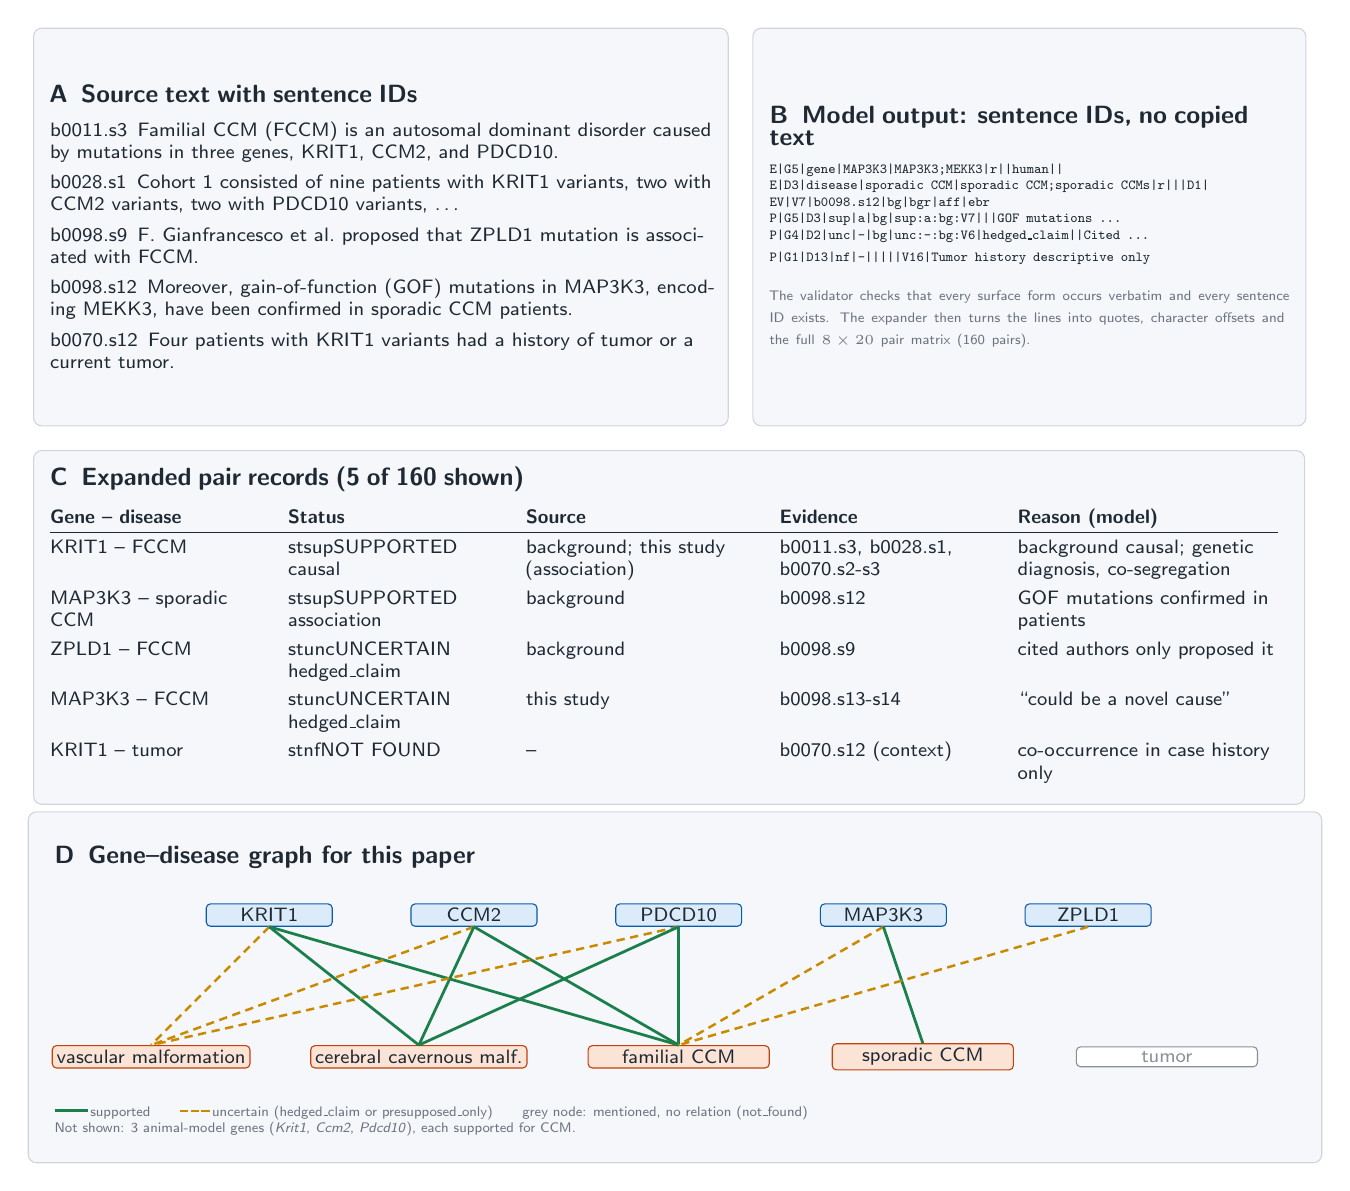
\begin{tikzpicture}[font=\sffamily\scriptsize, text=ink]
% ---------------- Panel A: source text
\node[panel, text width=8.4cm, minimum height=5.05cm, align=left, anchor=north west] (A) at (0,0) {%
  {\sffamily\bfseries\small A\enspace Source text with sentence IDs}\\[4pt]
  \fS{b0011.s3}\enspace \fD{Familial CCM (FCCM)} is an autosomal dominant disorder caused by mutations in three genes, \fG{KRIT1}, \fG{CCM2}, and \fG{PDCD10}.\\[3pt]
  \fS{b0028.s1}\enspace Cohort 1 consisted of nine patients with \fG{KRIT1} variants, two with \fG{CCM2} variants, two with \fG{PDCD10} variants, \dots\\[3pt]
  \fS{b0098.s9}\enspace F. Gianfrancesco et al.\ proposed that \fG{ZPLD1} mutation is associated with \fD{FCCM}.\\[3pt]
  \fS{b0098.s12}\enspace Moreover, gain-of-function (GOF) mutations in \fG{MAP3K3}, encoding \fG{MEKK3}, have been confirmed in \fD{sporadic CCM} patients.\\[3pt]
  \fS{b0070.s12}\enspace Four patients with \fG{KRIT1} variants had a history of \fD{tumor} or a current \fD{tumor}.};
% ---------------- Panel B: model output
\node[panel, text width=6.6cm, minimum height=5.05cm, align=left, anchor=north west] (B) at ($(A.north east)+(0.3,0)$) {%
  {\sffamily\bfseries\small B\enspace Model output: sentence IDs, no copied text}\\[4pt]
  {\ttfamily\tiny\color{ink}%
  E|G5|gene|MAP3K3|MAP3K3;MEKK3|r||human||\\
  E|D3|disease|sporadic CCM|sporadic CCM;sporadic CCMs|r|||D1|\\
  EV|V7|b0098.s12|bg|bgr|aff|ebr\\
  P|G5|D3|sup|a|bg|sup:a:bg:V7|||GOF mutations ...\\
  P|G4|D2|unc|-|bg|unc:-:bg:V6|hedged\_claim||Cited ...\\
  P|G1|D13|nf|-|||||V16|Tumor history descriptive only}\\[6pt]
  {\color{muted}\tiny The validator checks that every surface form occurs verbatim and every sentence ID exists. The expander then turns the lines into quotes, character offsets and the full $8\times20$ pair matrix (160 pairs).}};
% ---------------- Panel C: expanded pair table (spans both columns)
\path (A.south west) ++(0,-0.3) coordinate (Cnw);
\path (B.east) coordinate (Bx);
\node[panel, text width=15.72cm, align=left, anchor=north west] (C) at (Cnw) {%
  {\sffamily\bfseries\small C\enspace Expanded pair records (5 of 160 shown)}\\[3pt]
  \renewcommand{\arraystretch}{1.3}%
  \begin{tabular}{@{}p{2.6cm}p{2.6cm}p{2.8cm}p{2.6cm}p{3.3cm}@{}}
  \textbf{Gene -- disease} & \textbf{Status} & \textbf{Source} & \textbf{Evidence} & \textbf{Reason (model)}\\\hline
  \fG{KRIT1} -- \fD{FCCM} & \fst{stsup}{SUPPORTED} causal & background; this study (association) & \fS{b0011.s3, b0028.s1, b0070.s2-s3} & background causal; genetic diagnosis, co-segregation\\
  \fG{MAP3K3} -- \fD{sporadic CCM} & \fst{stsup}{SUPPORTED} association & background & \fS{b0098.s12} & GOF mutations confirmed in patients\\
  \fG{ZPLD1} -- \fD{FCCM} & \fst{stunc}{UNCERTAIN} hedged\_claim & background & \fS{b0098.s9} & cited authors only proposed it\\
  \fG{MAP3K3} -- \fD{FCCM} & \fst{stunc}{UNCERTAIN} hedged\_claim & this study & \fS{b0098.s13-s14} & ``could be a novel cause''\\
  \fG{KRIT1} -- \fD{tumor} & \fst{stnf}{NOT FOUND} & -- & \fS{b0070.s12} (context) & co-occurrence in case history only\\
  \end{tabular}};
% ---------------- Panel D: per-paper bipartite graph (human genes; 3 animal-model genes omitted)
\begin{scope}[shift={($(C.south west)+(0,-0.3)$)},
  gnode/.style={gene, minimum width=1.6cm, font=\sffamily\scriptsize},
  dnode/.style={dis, minimum width=2.3cm, font=\sffamily\scriptsize},
  sup/.style={draw=stsup, line width=1pt},
  unc/.style={draw=stunc, line width=0.9pt, densely dashed}]
\node[anchor=north west, font=\sffamily\bfseries\small] (Dt) at (0.15,-0.1) {D\enspace Gene--disease graph for this paper};
\foreach \g/\x in {KRIT1/3.0, CCM2/5.6, PDCD10/8.2, MAP3K3/10.8, ZPLD1/13.4}
  \node[gnode] (g-\g) at (\x,-1.1) {\g};
\node[dnode] (d-VM) at (1.5,-2.9) {vascular malformation};
\node[dnode] (d-CCM) at (4.9,-2.9) {cerebral cavernous malf.};
\node[dnode] (d-FCCM) at (8.2,-2.9) {familial CCM};
\node[dnode] (d-SCCM) at (11.3,-2.9) {sporadic CCM};
\node[dnode, fill=white, draw=stnf, text=stnf] (d-TUM) at (14.4,-2.9) {tumor};
\foreach \g in {KRIT1, CCM2, PDCD10} {
  \draw[unc] (g-\g.south) -- (d-VM.north);
  \draw[sup] (g-\g.south) -- (d-CCM.north);
  \draw[sup] (g-\g.south) -- (d-FCCM.north);
}
\draw[unc] (g-MAP3K3.south) -- (d-FCCM.north);
\draw[sup] (g-MAP3K3.south) -- (d-SCCM.north);
\draw[unc] (g-ZPLD1.south) -- (d-FCCM.north);
\node[anchor=north west, font=\sffamily\tiny, text=muted, align=left] (Dleg) at (0.15,-3.4)
  {\textcolor{stsup}{\rule[1.5pt]{12pt}{1pt}}\,supported\qquad
   \textcolor{stunc}{\rule[1.5pt]{3pt}{0.9pt}\,\rule[1.5pt]{3pt}{0.9pt}\,\rule[1.5pt]{3pt}{0.9pt}}\,uncertain (hedged\_claim or presupposed\_only)\qquad
   grey node: mentioned, no relation (not\_found)\\
   Not shown: 3 animal-model genes (\textit{Krit1}, \textit{Ccm2}, \textit{Pdcd10}), each supported for CCM.};
\end{scope}
\begin{scope}[on background layer]
  \node[panel, fit={(Dt) (Dleg) (d-TUM) ($(C.south east)+(0,-0.3)$)}] {};
\end{scope}
\end{tikzpicture}
}
\caption{Traceable extraction on one full-text article, PMC10014009~\cite{kim2023fccm}. (A)~Excerpts with stable sentence IDs; genes in blue, disease mentions in coral. (B)~The model's compact output cites sentence IDs only. (C)~Deterministically expanded pair records covering three statuses and both sources. (D)~The resulting per-paper bipartite graph. Quotes are reproduced from an open-access article (CC~BY-NC-ND~4.0) for illustration.}
\label{fig:example}
\end{figure}

\subsubsection{Comparators}
We compared our pipeline against two reference systems. First, we queried the public \emph{PubTator3} API~\cite{wei2024pubtator3} as a representative supervised literature system; because its relation extractor is trained on BioRED and operates on abstracts only (even for RENET2 full-text articles), it provides an in-domain supervised benchmark on BioRED and an abstract-only baseline on full texts. Second, to test whether extraction behaviour is tied to a single LLM family, we ran \emph{GPT-6.1 Sol} via the Codex CLI using the exact same frozen decision card, output format, packed text, and validator. \todo{add an open-weight LLM with the same card, and published supervised BioRED results as reference rows.}

\subsection{Evaluation}\label{sec:eval}
All systems and benchmarks were scored with the same script at the document-level (gene concept, disease concept) pair unit. A predicted entity aligns with a gold concept when any of its verbatim mentions overlaps a gold mention by character span within the same text block, allowing spelling variants to align without database normalization. We report precision, recall, and F1 with 95\% confidence intervals from a document-level bootstrap (2,000 resamples, seed 20261028)~\cite{efron1993bootstrap} because pairs within a document are not independent.

Because our output assigns graded statuses and reason codes, a single run supports three operating points: \emph{strict} (the default, counting only \st{supported} pairs as predictions), \emph{supported + uncertain} (counting all \st{uncertain} pairs as well), and \emph{supported + hedged/scope} (counting \st{uncertain} pairs only when their reason codes are limited to \st{hedged\_claim} and/or \st{scope}, chosen on BioRED Train+Dev and evaluated once on held-out Test). To quantify how much of the recall gap stems from excluding symptoms and general phenotypes as primary diseases, we also report a \emph{scope-adjusted view} that removes such gold pairs from the recall denominator alongside the strict view.

%% ===================================================================
\section{Results}

\subsection{Performance Comparison}
Table~\ref{tab:main} and Fig.~\ref{fig:pr} summarize extraction performance across all benchmarks. On the full set of 419 BioRED abstracts, 89\% of \st{supported} predictions matched gold relations, yielding strict precision of 0.894 and recall of 0.430 (F1 0.581). Performance was consistent across splits (F1 of 0.584 on Train, 0.608 on Dev, and 0.542 on Test), and the scope-adjusted view raised recall to 0.468 (F1 0.614).

Comparing our method with PubTator3 across the three benchmarks highlights their distinct operating characteristics. On the 50-abstract BioRED Test sample, where PubTator3 is evaluated in-domain, both systems reached similar precision (0.835 vs 0.827), while PubTator3 achieved higher recall (0.647 vs 0.412). Their predictions were complementary: among the 238 gold relations, 78 were found by both systems, 76 only by PubTator3, and 20 only by our method (with 64 missed by both), so their union recovered 174 relations (73\%). On out-of-domain EU-ADR abstracts, F1 was comparable (0.506 vs 0.529, overlapping intervals), reflecting higher precision for our method (0.469 vs 0.408) and higher recall for PubTator3 (0.754 vs 0.549). On the 40 RENET2 full texts, where PubTator3 is limited to abstracts, our method achieved higher recall (0.370 vs 0.254 in the strict view, rising to 0.464 when counting \st{uncertain} pairs).

Substituting GPT-6.1 Sol for Claude Opus 5.5 under the same frozen card yielded virtually identical results on the BioRED sample (F1 0.555 vs 0.551) and 0.986 pair-status agreement across 11 full texts.

\begin{table}[!htbp]
\centering\footnotesize
\caption{Main results, strict view unless stated. Brackets: 95\% bootstrap confidence intervals over documents.}
\label{tab:main}
\resizebox{\linewidth}{!}{%
\begin{tabular}{@{}llccc@{}}
\toprule
Benchmark (documents) & System / operating point & Precision & Recall & F1 [95\% CI]\\
\midrule
\multirow{2}{*}{BioRED, all (419)} & Ours & 0.894 [0.855, 0.931] & 0.430 & 0.581 [0.538, 0.625]\\
 & Ours, supported + uncertain & 0.814 & 0.577 & 0.676 [0.636, 0.714]\\
\addlinespace
\multirow{2}{*}{BioRED Test (73)} & Ours & 0.853 & 0.397 & 0.542 [0.444, 0.644]\\
 & Ours, supported + hedged/scope & 0.846 & 0.498 & 0.627\\
\addlinespace
\multirow{3}{*}{BioRED Test sample (50)} & Ours & 0.835 & 0.412 & 0.551 [0.440, 0.665]\\
 & Ours with GPT-6.1 Sol & 0.853 & 0.412 & 0.555 [0.465, 0.639]\\
 & PubTator3 & 0.827 & \textbf{0.647} & \textbf{0.726} [0.609, 0.825]\\
\addlinespace
\multirow{2}{*}{EU-ADR, PA (100)} & Ours & \textbf{0.469} [0.350, 0.600] & 0.549 & 0.506 [0.403, 0.602]\\
 & PubTator3 & 0.408 [0.326, 0.498] & \textbf{0.754} & 0.529 [0.447, 0.612]\\
\addlinespace
\multirow{3}{*}{RENET2 full text (40)} & Ours & 0.318 [0.206, 0.470] & 0.370 & 0.342 [0.258, 0.421]\\
 & Ours, supported + uncertain & 0.312 & \textbf{0.464} & 0.373\\
 & PubTator3 & \textbf{0.623} [0.511, 0.750] & 0.254 & 0.361 [0.243, 0.475]\\
\bottomrule
\end{tabular}}
\end{table}

\begin{figure}[!htbp]
\centering
\resizebox{\linewidth}{!}{% Figure 3. Precision-recall operating points with 95% bootstrap CIs.
% Values from experiments/single_shot/runs/*/*/{biored,euadr,renet2}_eval.json
% (Test hedged/scope point: experiments/single_shot/README.md, optimization round 1; no CI computed).
\newcommand{\isoFone}{%
  \foreach \F in {0.3,0.4,0.5,0.6,0.7,0.8} {
    \addplot[draw=rule, line width=0.5pt, dashed, domain=\F/2+0.02:0.95, samples=60, forget plot] {\F*x/(2*x-\F)};
  }
}
\newcommand{\isoLabels}{%
  % F1 contour labels, placed on each curve at recall 0.905
  \node[font=\sffamily\tiny, text=muted, anchor=south west, inner sep=1pt] at (axis cs:0.905,0.717) {F1=.8};
  \node[font=\sffamily\tiny, text=muted, anchor=south west, inner sep=1pt] at (axis cs:0.905,0.571) {.7};
  \node[font=\sffamily\tiny, text=muted, anchor=south west, inner sep=1pt] at (axis cs:0.905,0.449) {.6};
  \node[font=\sffamily\tiny, text=muted, anchor=south west, inner sep=1pt] at (axis cs:0.905,0.345) {.5};
  \node[font=\sffamily\tiny, text=muted, anchor=south west, inner sep=1pt] at (axis cs:0.905,0.257) {.4};
  \node[font=\sffamily\tiny, text=muted, anchor=south west, inner sep=1pt] at (axis cs:0.905,0.180) {.3};
}
\newcommand{\isoLabelsZoom}{%
  \node[font=\sffamily\tiny, text=muted, anchor=south west, inner sep=1pt] at (axis cs:0.83,0.772) {F1=.8};
  \node[font=\sffamily\tiny, text=muted, anchor=south west, inner sep=1pt] at (axis cs:0.83,0.605) {.7};
}
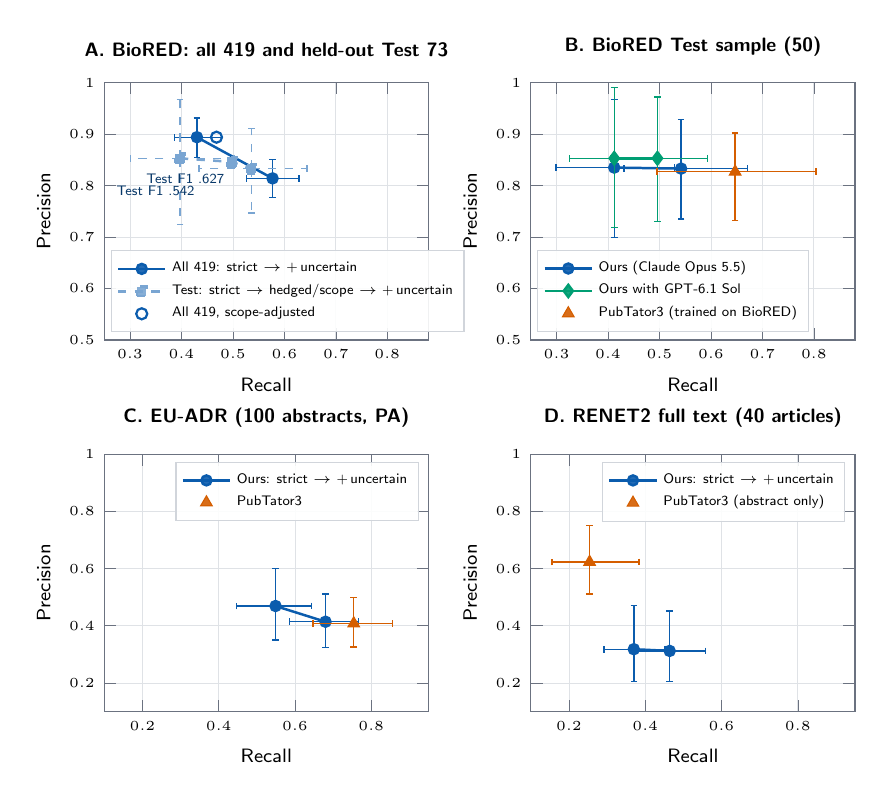
\begin{tikzpicture}
\begin{groupplot}[
  group style={group size=2 by 2, horizontal sep=1.3cm, vertical sep=1.45cm},
  gdt,
  width=0.47\linewidth, height=0.40\linewidth,
  xmin=0.1, xmax=0.95, ymin=0.1, ymax=1.0,
  xtick={0.2,0.4,0.6,0.8}, ytick={0.2,0.4,0.6,0.8,1.0},
  xlabel={Recall}, ylabel={Precision},
  clip mode=individual,
  error bars/error bar style={line width=0.5pt},
  error bars/error mark options={rotate=90, mark size=1.2pt, line width=0.5pt},
  legend style={font=\sffamily\tiny, draw=rule, fill=white, fill opacity=0.9, text opacity=1, row sep=-1pt, inner sep=2pt},
  legend cell align=left,
]
% ---------------- A: BioRED, all 419 and held-out Test 73
\nextgroupplot[title={A. BioRED: all 419 and held-out Test 73}, xmin=0.25, xmax=0.88, ymin=0.5, ymax=1.0, xtick={0.3,0.4,0.5,0.6,0.7,0.8}, ytick={0.5,0.6,0.7,0.8,0.9,1.0}, legend style={at={(0.02,0.03)}, anchor=south west}]
\isoFone
\addplot[ours, line width=0.9pt, mark=*, mark size=1.8pt,
  error bars/.cd, x dir=both, x explicit, y dir=both, y explicit]
  coordinates {
    (0.430,0.894) += (0.048,0.037) -= (0.044,0.039)
    (0.577,0.814) += (0.051,0.037) -= (0.051,0.037)
  };
\addlegendentry{All 419: strict $\rightarrow$ +\,uncertain}
\addplot[ours!55, line width=0.9pt, dashed, mark=square*, mark size=1.7pt,
  error bars/.cd, x dir=both, x explicit, y dir=both, y explicit]
  coordinates {
    (0.397,0.853) += (0.105,0.114) -= (0.096,0.128)
    (0.498,0.846) += (0,0) -= (0,0)
    (0.536,0.833) += (0.108,0.078) -= (0.102,0.086)
  };
\addlegendentry{Test: strict $\rightarrow$ hedged/scope $\rightarrow$ +\,uncertain}
\addplot[only marks, mark=o, mark size=2pt, draw=ours, line width=0.8pt] coordinates {(0.468,0.894)};
\addlegendentry{All 419, scope-adjusted}
\node[font=\sffamily\tiny, text=ours!60!black, anchor=north east, inner sep=2pt] at (axis cs:0.495,0.835) {Test F1 .627};
\node[font=\sffamily\tiny, text=ours!60!black, anchor=west, inner sep=2pt] at (axis cs:0.262,0.79) {Test F1 .542};
\isoLabelsZoom
% ---------------- B: BioRED 50-abstract Test sample
\nextgroupplot[title={B. BioRED Test sample (50)}, xmin=0.25, xmax=0.88, ymin=0.5, ymax=1.0, xtick={0.3,0.4,0.5,0.6,0.7,0.8}, ytick={0.5,0.6,0.7,0.8,0.9,1.0}, legend style={at={(0.02,0.03)}, anchor=south west}]
\isoFone
\addplot[ours, line width=0.9pt, mark=*, mark size=1.8pt,
  error bars/.cd, x dir=both, x explicit, y dir=both, y explicit]
  coordinates {
    (0.412,0.835) += (0.117,0.132) -= (0.113,0.136)
    (0.542,0.833) += (0.129,0.096) -= (0.111,0.098)
  };
\addlegendentry{Ours (Claude Opus 5.5)}
\addplot[gpt, line width=0.9pt, mark=diamond*, mark size=2.2pt,
  error bars/.cd, x dir=both, x explicit, y dir=both, y explicit]
  coordinates {
    (0.412,0.853) += (0.083,0.138) -= (0.087,0.135)
    (0.496,0.853) += (0.097,0.119) -= (0.090,0.123)
  };
\addlegendentry{Ours with GPT-6.1 Sol}
\addplot[only marks, pubtator, mark=triangle*, mark size=2.4pt,
  error bars/.cd, x dir=both, x explicit, y dir=both, y explicit]
  coordinates {(0.647,0.827) += (0.157,0.075) -= (0.152,0.095)};
\addlegendentry{PubTator3 (trained on BioRED)}
\isoLabelsZoom
% ---------------- C: EU-ADR, positive associations
\nextgroupplot[title={C. EU-ADR (100 abstracts, PA)}, legend pos=north east]
\isoFone
\addplot[ours, line width=0.9pt, mark=*, mark size=1.8pt,
  error bars/.cd, x dir=both, x explicit, y dir=both, y explicit]
  coordinates {
    (0.549,0.469) += (0.095,0.131) -= (0.102,0.119)
    (0.680,0.414) += (0.086,0.097) -= (0.095,0.090)
  };
\addlegendentry{Ours: strict $\rightarrow$ +\,uncertain}
\addplot[only marks, pubtator, mark=triangle*, mark size=2.4pt,
  error bars/.cd, x dir=both, x explicit, y dir=both, y explicit]
  coordinates {(0.754,0.408) += (0.101,0.090) -= (0.107,0.082)};
\addlegendentry{PubTator3}
\isoLabels
% ---------------- D: RENET2 full text
\nextgroupplot[title={D. RENET2 full text (40 articles)}, legend pos=north east]
\isoFone
\addplot[ours, line width=0.9pt, mark=*, mark size=1.8pt,
  error bars/.cd, x dir=both, x explicit, y dir=both, y explicit]
  coordinates {
    (0.370,0.318) += (0.082,0.152) -= (0.078,0.112)
    (0.464,0.312) += (0.094,0.140) -= (0.084,0.106)
  };
\addlegendentry{Ours: strict $\rightarrow$ +\,uncertain}
\addplot[only marks, pubtator, mark=triangle*, mark size=2.4pt,
  error bars/.cd, x dir=both, x explicit, y dir=both, y explicit]
  coordinates {(0.254,0.623) += (0.130,0.127) -= (0.099,0.112)};
\addlegendentry{PubTator3 (abstract only)}
\isoLabels
\end{groupplot}
\end{tikzpicture}
}
\caption{Precision and recall of each system and operating point, with 95\% bootstrap confidence intervals over documents. Dashed grey curves are F1 contours from 0.3 to 0.8 in steps of 0.1; panels A and B are zoomed to precision $\geq 0.5$. Connected points are operating points of one run: strict (supported only) and adding uncertain pairs; in panel A, the middle Test point is the hedged/scope operating point chosen on Train+Dev (no interval computed). On EU-ADR and RENET2, measured precision is a lower bound because the gold sets are incomplete.}
\label{fig:pr}
\end{figure}

\subsection{Status Labels Against Graded Gold Labels}
Benchmarks with graded, negative, or novelty annotations allow evaluation of our status and source labels beyond binary matching. On EU-ADR, our method labelled all 3 gold negative (NA) pairs as \st{explicit\_negative}, whereas PubTator3 misclassified one as positive. Across the 122 positive (PA) pairs, our method labelled 67 \st{supported}, 16 \st{uncertain}, 10 \st{not\_found}, and 4 \st{explicit\_negative}, while 25 involved an endpoint not recorded as a primary entity; counting \st{uncertain} pairs raised PA recall from 0.549 to 0.680 at 0.414 precision. On RENET2, only 2 of our 223 \st{supported} predictions conflicted with a silver non-associated label. On BioRED, our source label agreed with the gold \emph{Novel} label on 526 of 703 matched relations (75\%).

Within the \st{uncertain} status, the required reason codes separated pairs that benchmark annotators consider positive from those they do not (Fig.~\ref{fig:recall}B). On BioRED Train+Dev, the share of \st{uncertain} pairs matching a gold relation was 82\% for \st{hedged\_claim} alone ($n=99$), 75\% for \st{hedged\_claim} + \st{scope} ($n=32$), and 62\% for \st{scope} alone ($n=113$), versus 38\% for \st{presupposed\_only} and 6\% for \st{identity}. Counting only the first three groups as positive predictions raised held-out BioRED Test F1 from 0.542 to 0.627, lifting recall from 0.397 to 0.498 at unchanged precision (0.846 vs 0.853) with no extra model calls.

\subsection{Error Analysis}

\subsubsection{Missed Relations}
To understand the recall gap on BioRED, we audited all 930 gold relations missed under the strict view (Fig.~\ref{fig:recall}A). Nearly three-fifths (547 relations, 59\%) were pairs whose endpoints the model extracted and explicitly judged as non-supported: 295 were assigned \st{not\_found}, 240 \st{uncertain}, and 12 \st{explicit\_negative}. The remaining 383 misses (41\%) stemmed from entity-scope boundaries: 131 involved disease mentions recorded as auxiliary symptoms or phenotypes, while 159 diseases and 93 genes were not extracted as primary entities. On Train+Dev, these unrecorded mentions consisted mainly of gene families or protein complexes (e.g.\ NF-$\kappa$B, MAPK, Wnt, and NMDA receptors), which our decision card excludes as single-gene endpoints, alongside broad disease terms such as ``cancer'', ``tumor'', and ``inflammation''. Even if all such broad gene and disease mentions were extracted and judged \st{supported}, overall recall would increase by at most 4.0 and 6.6 percentage points, respectively.

Because 117 of the 155 unjudged gold relations on Train+Dev (75\%) had both entities in the same sentence, we ran two targeted experiments on the Dev split (71 abstracts) to test whether the model was overlooking co-mentioned pairs. First, prompt variant V4 required the model to output an explicit judgment for every co-mentioned pair; instead of improving recall, this constraint lowered recall from 0.454 to 0.403, reduced \st{supported} predictions from 153 to 133, raised precision from 0.922 to 0.947, and increased API cost by 16\%. Second, we extracted all 97 unjudged same-sentence pairs across 18 Dev abstracts and prompted the model in a separate request to judge each pair directly: 92 remained \st{not\_found}, 4 became \st{uncertain}, 1 became \st{explicit\_negative}, and none became \st{supported}, leaving all evaluation metrics unchanged at an added cost of USD 0.64. Thus, even when directed to the exact sentence and entity pair, the model judged that the text did not satisfy the decision card's criteria for a supported relation, confirming that the recall gap reflects a stricter evidence threshold rather than missed text.

\begin{figure}[!htbp]
\centering
\resizebox{\linewidth}{!}{% Figure 4. Where BioRED recall is lost (A) and which uncertain pairs are worth counting (B).
% A: 930 missed gold relations, all 419 abstracts (experiments/biored/README.md).
% B: share of uncertain pairs that are gold relations by reason code, Train+Dev
%    (experiments/single_shot/README.md, optimization round 1).
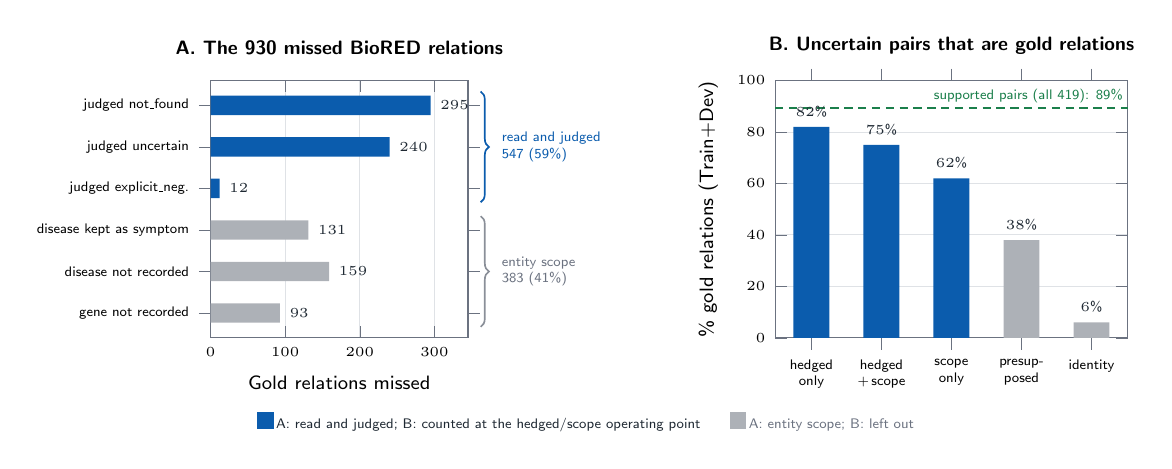
\begin{tikzpicture}
\begin{axis}[
  gdt, name=A, clip=false,
  title={A. The 930 missed BioRED relations},
  xbar, bar width=7pt, bar shift=0pt,
  width=0.40\linewidth, height=0.40\linewidth,
  xmin=0, xmax=345, xtick={0,100,200,300}, xlabel={Gold relations missed},
  y dir=reverse,
  symbolic y coords={nf,unc,neg,sym,dis,gen},
  ytick={nf,unc,neg,sym,dis,gen},
  yticklabels={judged not\_found, judged uncertain, judged explicit\_neg., disease kept as symptom, disease not recorded, gene not recorded},
  yticklabel style={font=\sffamily\tiny, align=right},
  ymajorgrids=false,
  nodes near coords, nodes near coords style={font=\sffamily\tiny, text=ink},
  enlarge y limits=0.12,
]
\addplot[fill=ours, draw=none] coordinates {(295,nf) (240,unc) (12,neg)};
\addplot[fill=stnf!70, draw=none] coordinates {(131,sym) (159,dis) (93,gen)};
\draw[decorate, decoration={brace, amplitude=3pt}, draw=ours, line width=0.6pt]
  ([yshift=5pt]axis cs:362,nf) -- ([yshift=-5pt]axis cs:362,neg)
  node[midway, right=4pt, font=\sffamily\tiny, text=ours, align=left] {read and judged\\547 (59\%)};
\draw[decorate, decoration={brace, amplitude=3pt}, draw=stnf, line width=0.6pt]
  ([yshift=5pt]axis cs:362,sym) -- ([yshift=-5pt]axis cs:362,gen)
  node[midway, right=4pt, font=\sffamily\tiny, text=muted, align=left] {entity scope\\383 (41\%)};
\end{axis}
\begin{axis}[
  gdt, at={(A.east)}, anchor=west, xshift=3.9cm,
  title={B. Uncertain pairs that are gold relations},
  ybar, bar width=13pt, bar shift=0pt,
  width=0.50\linewidth, height=0.40\linewidth,
  ymin=0, ymax=100, ylabel={\% gold relations (Train+Dev)},
  symbolic x coords={hed,hs,sco,pre,ide},
  xtick={hed,hs,sco,pre,ide},
  xticklabels={hedged\\only, hedged\\+\,scope, scope\\only, presup-\\posed, identity},
  xticklabel style={font=\sffamily\tiny, align=center},
  xmajorgrids=false,
  nodes near coords={\pgfmathprintnumber{\pgfplotspointmeta}\%},
  nodes near coords style={font=\sffamily\tiny, text=ink},
  enlarge x limits=0.13,
]
\addplot[fill=ours, draw=none] coordinates {(hed,82) (hs,75) (sco,62)};
\addplot[fill=stnf!70, draw=none] coordinates {(pre,38) (ide,6)};
\draw[densely dashed, draw=stsup, line width=0.7pt] (rel axis cs:0,0.894) -- (rel axis cs:1,0.894)
  node[pos=1, anchor=south east, font=\sffamily\tiny, text=stsup, inner sep=1.5pt] {supported pairs (all 419): 89\%};
\end{axis}
\node[font=\sffamily\tiny, anchor=north] at ($(current bounding box.south)+(0,-0.05cm)$)
  {\textcolor{ours}{\rule{6pt}{6pt}}\,\textcolor{ink}{A: read and judged; B: counted at the hedged/scope operating point}\qquad
   \textcolor{stnf!70}{\rule{6pt}{6pt}}\,\textcolor{muted}{A: entity scope; B: left out}};
\end{tikzpicture}
}
\caption{(A)~The 930 BioRED gold relations missed in the strict view (all 419 abstracts); most were read and judged by the model rather than overlooked. (B)~Share of \st{uncertain} pairs on Train+Dev that are gold relations, by reason code. Pairs with only \st{hedged\_claim} and/or \st{scope} reasons (blue) are counted at the hedged/scope operating point, which raised held-out Test F1 from 0.542 to 0.627.}
\label{fig:recall}
\end{figure}

\subsubsection{Extra Predictions}
We also examined the \st{supported} predictions counted as false positives across each benchmark. On BioRED, the 87 extra predictions fell into three categories: in 60 cases, BioRED annotated both concepts in the abstract but no relation between them; in 23 cases, our disease endpoint (such as a clinical outcome) was not annotated as a BioRED disease concept; and in 4 cases, our gene endpoint did not match a BioRED gene concept. On EU-ADR, 10 of our 37 extra predictions involving gold concepts had in fact been marked as positive by one annotator, falling just short of the multi-annotator consensus threshold. On RENET2, among our 152 \st{supported} predictions outside the gold positive set, 105 had never been evaluated because no baseline tool had proposed them, 45 involved an entity outside RENET2's concept vocabulary, and only 2 carried a silver non-associated label. Notably, 136 of these 152 extra predictions were relations our method tagged as \st{background}; measured precision on RENET2 was 0.53 for relations tagged \st{this study} versus 0.28 for \st{background} relations, matching RENET2's focus on curating main study findings rather than background literature.

\subsection{Full-Text Extraction and Cost}
On the 100-paper unlabelled PMC full-text corpus, our pipeline extracted 972 \st{supported} relations, 451 \st{uncertain} pairs, and 47 \st{explicit\_negative} pairs, compared with 198 relations reported by PubTator3. Among the 972 \st{supported} relations, 875 (90\%) were supported solely by sentences in the article body outside the abstract. Twenty-five papers yielded no \st{supported} relations: 8 contained no gene mentions, 8 contained no disease mentions, and 9 contained only co-occurrences, diagnostic gene-panel listings, or speculative statements. At list API prices, including validation repair calls, total extraction cost was USD 0.056 per BioRED abstract, USD 4.75 across the 100 EU-ADR abstracts, USD 6.36 across the 40 RENET2 articles, and USD 0.44 per full-text paper, with a mean generation time of 78\,s per full text. \todo{annotate 15--20 of these papers to measure full-text precision and recall.}

%% ===================================================================
\section{Discussion}

\subsection{Why the Benchmarks Disagree}
Although the exact same frozen pipeline was applied without modification across all datasets, strict F1 varied from 0.58 on BioRED to 0.51 on EU-ADR and 0.34 on RENET2. This spread directly reflects differences in how each benchmark defines and labels relations. BioRED annotates all relations stated in an abstract, including hedged statements, and groups symptoms, phenotypes, and broad terms such as ``cancer'' under its disease category. EU-ADR retains only relations endorsed by at least two annotators. RENET2 labels only candidate pairs proposed by its text-mining tools and assigns negative labels automatically without manual verification. A precision-oriented extractor governed by fixed rules is therefore penalized differently under each protocol, and on incomplete gold sets such as EU-ADR and RENET2 its measured precision represents a lower bound~\cite{wadhwa2023revisiting,fan2024evaluating}. Crucially, across the two corpora that include negative labels, our method rarely contradicted an explicit negative annotation, matching 0 of 3 negative pairs on EU-ADR and only 2 of 223 \st{supported} pairs on RENET2. Most apparent false positives are thus unannotated mentions or background citations rather than factual contradictions, which is the distinction that matters when a human curator audits the cited evidence sentences.

\subsection{Implications for Curation}
Assigning four-way statuses and reason codes in a single pass allows one extraction run to serve different curation workflows. An automated knowledge-base pipeline can ingest \st{supported} pairs directly while routing \st{uncertain} pairs tagged \st{hedged\_claim} or \st{scope} to human review; on held-out BioRED Test abstracts, including this subset recovered 10 percentage points of recall at virtually no cost to precision. Standard binary classifiers, by contrast, cannot separate hedged scientific claims from entity-identity ambiguities without retraining.

Our results also show that rule-guided LLM extraction complements supervised systems. PubTator3 achieves higher recall within its BioRED training domain, whereas our pipeline extracts evidence from the full text, separates study findings from background citations, and flags explicit negative findings. On the BioRED sample, combining both systems recovered 73\% of gold relations compared with 65\% for PubTator3 alone, pointing to a practical hybrid architecture in which a fast supervised extractor proposes candidate pairs and our decision-card pipeline verifies each candidate with sentence-level evidence. Moreover, because the decision card is human-readable and version-controlled, adapting the extractor to a new relation type (such as chemical--disease associations) requires editing a one-page specification rather than re-annotating a training corpus. The near-identical performance of GPT-6.1 Sol further indicates that extraction behaviour is governed by the written rules rather than a single proprietary model.

\subsection{Limitations}
Several limitations warrant consideration. First, we have not yet conducted dual-annotator adjudication of the extra predictions; our interpretation that many apparent false positives are valid unannotated relations relies on each benchmark's annotation structure (such as single-annotator labels in EU-ADR and background citations in RENET2) and spot checks rather than formal manual review. Second, the RENET2 evaluation (40 articles) and the BioRED head-to-head comparison with PubTator3 (50 abstracts) used moderate sample sizes, resulting in wide confidence intervals on some metrics, and we did not perform paired significance tests. Third, entities are aligned by verbatim character spans rather than normalized to NCBI Gene or MeSH identifiers, which currently prevents cross-document aggregation and direct database comparison with DisGeNET~\cite{pinero2020disgenet} or CTD~\cite{davis2023ctd}. Fourth, both Claude Opus 5.5 and GPT-6.1 Sol are proprietary models subject to version changes; to support reproducibility, we archive all prompts, raw model outputs, and evaluation scripts. Fifth, public benchmark abstracts may overlap with LLM pretraining corpora, just as BioRED was used to train PubTator3. Sixth, each benchmark configuration was executed once; although pair-status agreement of 0.976--0.985 across development runs indicates high stability, we did not quantify run-to-run variance across the full benchmarks. Finally, our 100-paper full-text corpus lacks gold-standard annotations, and the released RENET2 texts are truncated to the early body.

%% ===================================================================
\section{Conclusions}
By pairing a frozen, one-page decision card with sentence-ID citations and deterministic validation, a general-purpose LLM can extract gene--disease relations from full-text articles with verbatim sentence evidence, four-way certainty statuses, and source labels in a single request at USD 0.44 per paper. Evaluated without tuning across three benchmarks with distinct annotation protocols, the method achieved high precision on BioRED (0.894) and rarely contradicted explicit negative labels on EU-ADR or RENET2. Targeted re-querying of unjudged same-sentence pairs produced no additional supported relations, demonstrating that the recall gap stems from a stricter evidence standard rather than overlooked text, while routing \st{uncertain} pairs by reason code recovered 10 recall points on held-out data without precision loss. Future work will incorporate dual-annotator adjudication of extra predictions, concept normalization to NCBI Gene and MeSH, and hybrid pipelines that combine supervised candidate generation with decision-card verification.

%% ===================================================================
\section*{CRediT authorship contribution statement}
\todo{to be agreed with co-authors}

\section*{Declaration of competing interest}
\todo{to complete}

\section*{Data and code availability}
Code, the decision card, prompts, raw model outputs and scoring scripts will be released at \todo{repository URL}. EU-ADR and RENET2 texts are not redistributed; download scripts are provided.

\section*{Declaration of generative AI use}
\todo{Required by the publisher. Describe the use of AI tools in drafting this manuscript; check the current Elsevier wording.}

\section*{Acknowledgements}
\todo{funding and acknowledgements}

\bibliographystyle{elsarticle-num}
\bibliography{refs}

\end{document}
